% appendixd.tex
% Dieses Werk ist unter einem Creative Commons Namensnennung-Keine kommerzielle Nutzung-Weitergabe 
% unter gleichen Bedingungen 3.0 Deutschland Lizenzvertrag lizenziert. Um die Lizenz anzusehen, gehen Sie bitte 
% zu http://creativecommons.org/licenses/by-nc-sa/3.0/de/ oder schicken Sie einen Brief an 
% Creative Commons, 171 Second Street, Suite 300, San Francisco, California 94105, USA.


\chapter{Answers to ``Things to try''}\label{app:answers}

Here is where you can find the answers to the questions asked in each chapter in the section ``Things to try''.

\subsection*{Chapter \ref{ch:8multipliedby3.57}}

1. The answer to \textbf{Exercise 1} might be something like the following:

\begin{listing}
\begin{verbatim}
>>> toys = [ 'car', 'Nintendo Wii', 'computer', 'bike' ]
>>> foods = [ 'pancakes', 'chocolate', 'ice cream' ]
>>> favourites = toys + foods
>>> print(favourites)
['car', 'Nintendo Wii', 'computer', 'bike', 'pancakes', 'chocolate', 'ice cream']
\end{verbatim}
\end{listing}

\noindent
2.  The answer to \textbf{Exercise 2} is simply adding the result of multiplying 3 by 25 and the result of multiplying 10 by 32.  The following equations shows the result of this equation:

\begin{listing}
\begin{verbatim}
>>> print(3 * 25 + 10 * 32)
395
\end{verbatim}
\end{listing}

\noindent
However, given that we looked at the use of brackets in Chapter 2, you might have decided that you needed to put brackets around some parts of this equation.  You might've done something like this:

\begin{listing}
\begin{verbatim}
>>> print((3 * 25) + (10 * 32))
395
\end{verbatim}
\end{listing}

\noindent
The answer is the same, because multiplication is done before addition.  In either equation, the two multiplication operations are performed first, and the results are added.  However, the second equation is possibly slightly better than the first---because it's immediately obvious to the reader which operations are performed first.  A less knowledgeable programmer (who doesn't know as much about the order of operations) might think that, in the first equation, you multiply 3 by 25, then add 10, then multiply the result by 32 (the answer to that is 2720---completely wrong).  With the brackets, it's a bit more obvious what gets calculated first.

\noindent
3.  The answer to \textbf{Exercise 3} will be something like the following:

\begin{listing}
\begin{verbatim}
>>> first_name = 'Mary'
>>> second_name = 'Wilson'
>>> print('My name is %s %s' % (first_name, second_name))
My name is Mary Wilson
\end{verbatim}
\end{listing}

\subsection*{Chapter \ref{ch:turtles}}

\noindent
1. A rectangle is like a square, except two of its sides are longer than the other two.  By telling the turtle to do the following operations, you can easily draw a rectangle:

\begin{itemize}
 \item move forward a certain number of pixels
 \item turn left
 \item move forward a shorter number of pixels
 \item turn left
 \item move forward, the number of pixels in the first movement
 \item turn left
 \item move forward the shorter number of pixels in the second movement
\end{itemize}

\noindent
For example, the following code will drawing the rectangle in figure\ref{fig46}.

\begin{listing}
\begin{verbatim}
>>> import turtle
>>> t = turtle.Pen()
>>> t.forward(150)
>>> t.left(90)
>>> t.forward(50)
>>> t.left(90)
>>> t.forward(150)
>>> t.left(90)
>>> t.forward(50)
\end{verbatim}
\end{listing}

\begin{figure}
\begin{center}
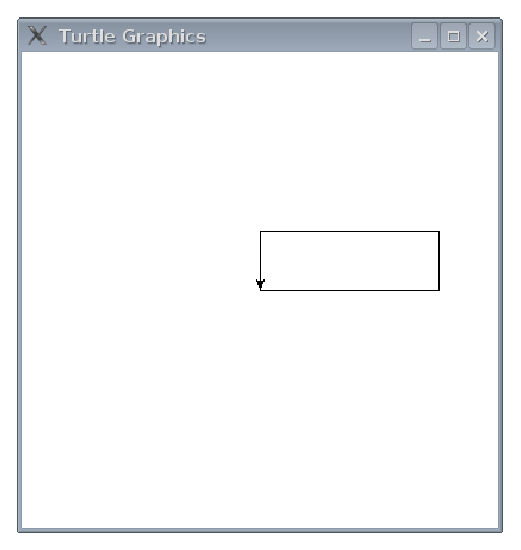
\includegraphics[width=82mm]{figure46.eps}
\end{center}
\caption{Turtle drawing a rectangle.}\label{fig46}
\end{figure}

\noindent
2. A triangle is a bit more complicated to draw, because you need to know more about angles and line lengths.  If you haven't studied angles in school then this may be a bit harder to do than you expect.  You can draw a basic triangle (see figure~\ref{fig47}) using the following code:

\begin{listing}
\begin{verbatim}
>>> import turtle
>>> t = turtle.Pen()
>>> t.forward(100)
>>> t.left(135)
>>> t.forward(70)
>>> t.left(90)
>>> t.forward(70)
\end{verbatim}
\end{listing}

\begin{figure}
\begin{center}
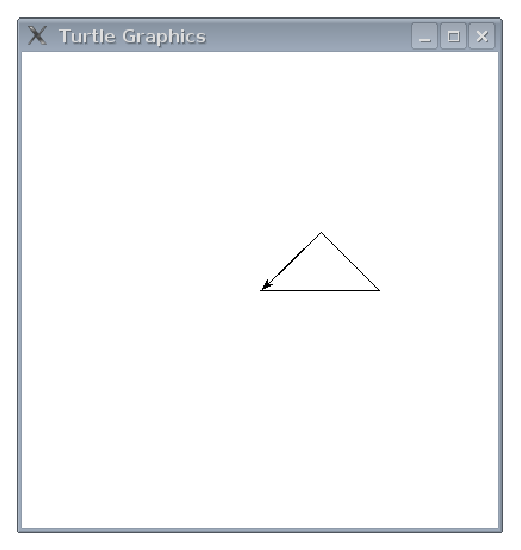
\includegraphics[width=82mm]{figure47.eps}
\end{center}
\caption{Turtle drawing a triangle.}\label{fig47}
\end{figure}


\subsection*{Chapter \ref{ch:againandagain}}

\noindent
1. The loop stops after the first print.  So when you run the code in the Python console you get:

\begin{listing}
\begin{verbatim}
>>> for x in range(0, 20):
...     print('hello %s' % x)
...     if x < 9:
...         break
hello 0
\end{verbatim}
\end{listing}

\noindent
The reason it stops after the first print is that during the first run of the loop, the value of the variable \code{x} is zero.  Since zero is less than nine, the break statement stops the loop from running any further.

\noindent
2. To figure out how much money you get when you are paid 3\% interest, you need to multiply the number by 0.03.  To begin with we should create a variable and point it at the amount of our savings:

\begin{listing}
\begin{verbatim}
>>> amount = 100
\end{verbatim}
\end{listing}

To the amount of interest paid for 1 year would be that amount multiplied by 0.03:

\begin{listing}
\begin{verbatim}
>>> amount = 100
>>> print(amount * 0.03)
3.0
\end{verbatim}
\end{listing}

That's \$3!  Not bad since we didn't need to do anything to get it.  We need to print out this value and then add it to the total, and do it 10 times to work out the interest that we are paid for 10 years:

\begin{listing}
\begin{verbatim}
>>> amount = 100
>>> for year in range(1, 11):
...     interest = amount * 0.03
...     print('interest earned for year %s is %s' % (year, interest))
...     amount = amount + interest
... 
interest earned for year 1 is 3.0
interest earned for year 2 is 3.09
interest earned for year 3 is 3.1827
interest earned for year 4 is 3.278181
interest earned for year 5 is 3.37652643
interest earned for year 6 is 3.4778222229
interest earned for year 7 is 3.58215688959
interest earned for year 8 is 3.68962159627
interest earned for year 9 is 3.80031024416
interest earned for year 10 is 3.91431955149
\end{verbatim}
\end{listing}

In the first line we create a for-loop using the variable \code{year} and the function \code{range} to count from 1 to 10.  The second line calculates the interest, multiplying the value in variable \code{amount} by 0.03.  The next line is the print statement---which uses place holders (\code{\%s}) to include the values for \code{year} and \code{interest}.  Finally in the last line, we add the interest back into the amount.
All the decimal places---the numbers after the period (.) in the print lines---are a bit confusing, but you can tell that the amount of interest each year increases a little bit as you add the interest.
The code might be a bit more helpful if we also add the total saved each year:

\begin{listing}
\begin{verbatim}
>>> amount = 100
>>> for year in range(1, 11):
...     interest = amount * 0.03
...     print('interest earned for savings %s for year %s is %s' % 
...         (amount, year, interest))
...     amount = amount + interest
... 
interest earned for savings 100 for year 1 is 3.0
interest earned for savings 103.0 for year 2 is 3.09
interest earned for savings 106.09 for year 3 is 3.1827
interest earned for savings 109.2727 for year 4 is 3.278181
interest earned for savings 112.550881 for year 5 is 3.37652643
interest earned for savings 115.92740743 for year 6 is 3.4778222229
interest earned for savings 119.405229653 for year 7 is 3.58215688959
interest earned for savings 122.987386542 for year 8 is 3.68962159627
interest earned for savings 126.677008139 for year 9 is 3.80031024416
interest earned for savings 130.477318383 for year 10 is 3.91431955149
\end{verbatim}
\end{listing}

\subsection*{Chapter \ref{ch:sortoflikerecycling}}

\noindent
1. Turning the for-loop into a function is actually quite easy.  The function will look something like this:

\begin{listing}
\begin{verbatim}
>>> def calculate_interest(amount, rate):
...     for year in range(1, 11):
...         interest = amount * rate
...         print('interest earned for savings %s for year %s is %s' % 
...             (amount, year, interest))
...         amount = amount + interest
\end{verbatim}
\end{listing}

If you compare the function with the code above, you might notice that, apart from the first line, there's only one change to the original code (0.03 is now the parameter \code{rate}). Because \code{amount} was already a variable, there's no change required when it becomes a parameter. You'll find the output is also the same when you run the function:

\begin{listing}
\begin{verbatim}
>>> calculate_interest(100, 0.03)
interest earned for savings 100 for year 1 is 3.0
interest earned for savings 103.0 for year 2 is 3.09
interest earned for savings 106.09 for year 3 is 3.1827
interest earned for savings 109.2727 for year 4 is 3.278181
interest earned for savings 112.550881 for year 5 is 3.37652643
interest earned for savings 115.92740743 for year 6 is 3.4778222229
interest earned for savings 119.405229653 for year 7 is 3.58215688959
interest earned for savings 122.987386542 for year 8 is 3.68962159627
interest earned for savings 126.677008139 for year 9 is 3.80031024416
interest earned for savings 130.477318383 for year 10 is 3.91431955149
\end{verbatim}
\end{listing}

\noindent
2. Changing the function to pass in the year as a parameter also involves only minor changes:

\begin{listing}
\begin{verbatim}
>>> def calculate_interest(amount, rate, years):
...     for year in range(1, years):
...         interest = amount * rate
...         print('interest earned for savings %s for year %s is %s' %
...             (amount, year, interest))
...         amount = amount + interest
\end{verbatim}
\end{listing}

\noindent
We can now easily change the starting amount, the rate of interest and the number of years:

\begin{listing}
\begin{verbatim}
>>> calculate_interest(1000, 0.05, 6)
interest earned for savings 1000 for year 1 is 50.0
interest earned for savings 1050.0 for year 2 is 52.5
interest earned for savings 1102.5 for year 3 is 55.125
interest earned for savings 1157.625 for year 4 is 57.88125
interest earned for savings 1215.50625 for year 5 is 60.7753125
\end{verbatim}
\end{listing}

\noindent
3. The mini-program is a bit more complicated than the functions we've already created.  First we need to import the sys module so we can ask for input.  Then we need to prompt the user of our program for each of the values.  Apart from that, the function stays roughly the same:

\begin{listing}
\begin{verbatim}
>>> import sys
>>> def calculate_interest():
...     print('Enter the amount you have to save')
...     amount = float(sys.stdin.readline())
...     print('Enter the interest rate')
...     rate = float(sys.stdin.readline())
...     print('Enter the number of years')
...     years = int(sys.stdin.readline())
...     for year in range(1, years):
...         interest = amount * rate
...         print('interest earned for savings %s for year %s is %s' % 
...             (amount, year, interest))
...         amount = amount + interest
\end{verbatim}
\end{listing}

\noindent
When we run the function, we'll see something like the following:

\begin{listingignore}
\begin{verbatim}
>>> calculate_interest()
Enter the amount you have to save
500
Enter the interest rate
0.06
Enter the number of years
12
interest earned for savings 500.0 for year 1 is 30.0
interest earned for savings 530.0 for year 2 is 31.8
interest earned for savings 561.8 for year 3 is 33.708
interest earned for savings 595.508 for year 4 is 35.73048
interest earned for savings 631.23848 for year 5 is 37.8743088
interest earned for savings 669.1127888 for year 6 is 40.146767328
interest earned for savings 709.259556128 for year 7 is 42.5555733677
interest earned for savings 751.815129496 for year 8 is 45.1089077697
interest earned for savings 796.924037265 for year 9 is 47.8154422359
interest earned for savings 844.739479501 for year 10 is 50.6843687701
interest earned for savings 895.423848271 for year 11 is 53.7254308963
\end{verbatim}
\end{listingignore}

\subsection*{Chapter \ref{ch:turtlesgalore}}

\noindent
1. There's a hard way to draw an octagon, and an easy way.  The hard way, isn't hard because it's complicated.  It's hard because it requires more typing:

\begin{listing}
\begin{verbatim}
import turtle
t = turtle.Pen()
>>> t.forward(50)
>>> t.right(45)
>>> t.forward(50)
>>> t.right(45)
>>> t.forward(50)
>>> t.right(45)
>>> t.forward(50)
>>> t.right(45)
>>> t.forward(50)
>>> t.right(45)
>>> t.forward(50)
>>> t.right(45)
>>> t.forward(50)
>>> t.right(45)
>>> t.forward(50)
\end{verbatim}
\end{listing}

\noindent
You can see from that code that we tell the turtle to move forward 50 pixels, then turn right 45 degrees.  We do this 8 times.  Which is a lot of time.  The easier way to draw an octagon is the following code (which produces the octagon in figure~\ref{fig48}):

\begin{listing}
\begin{verbatim}
>>> for x in range(0,8):
...     t.forward(50)
...     t.right(45)
\end{verbatim}
\end{listing}

\begin{figure}
\begin{center}
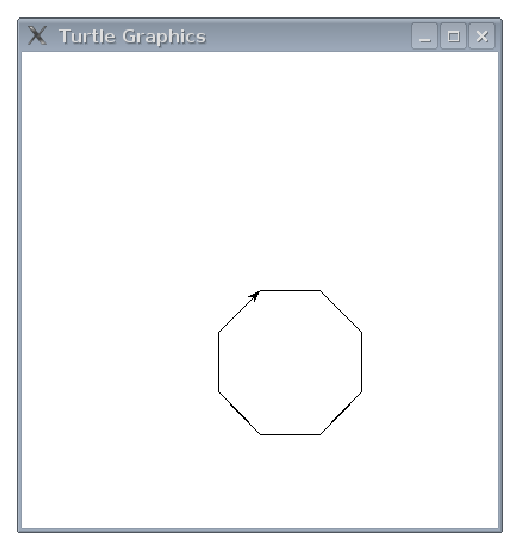
\includegraphics[width=82mm]{figure48.eps}
\end{center}
\caption{Turtle drawing an octagon.}\label{fig48}
\end{figure}

\noindent
2.  If you take another look at the other functions in Chapter~\ref{ch:turtlesgalore}, you'll already see how to create a filled shape. We can convert the octagon code into a function that takes a colour, but we'll also want to reuse the hexcolour function 

\begin{listing}
\begin{verbatim}
>>> def octagon(red, green, blue):
...     t.color(red, green, blue)
...     t.begin_fill()
...     for x in range(0,8):
...         t.forward(50)
...         t.right(45)
...     t.end_fill()
\end{verbatim}
\end{listing}

We set the colour, then turn filling on.  Then we run the for loop to draw the octagon, finally we switch filling back off again to fill in the shape. How about a blue octagon (see figure~\ref{fig49}):

\begin{listing}
\begin{verbatim}
>>> octagon(0, 0, 1)
\end{verbatim}
\end{listing}

\begin{figure}
\begin{center}
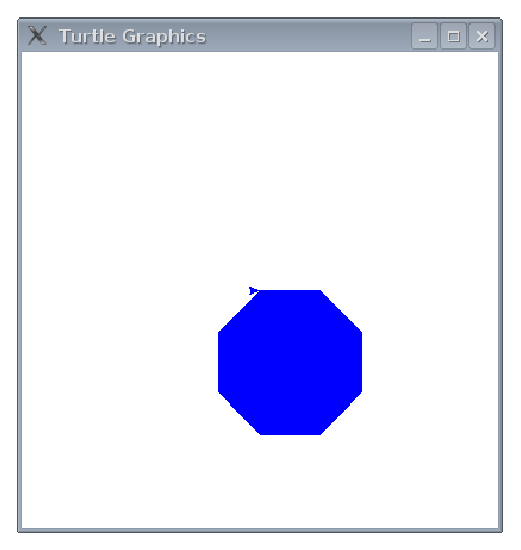
\includegraphics[width=82mm]{figure49.eps}
\end{center}
\caption{Turtle drawing a blue octagon.}\label{fig49}
\end{figure}
\newpage
